% The entire content of this work (including the source code
% for TeX files and the generated PDF documents) by 
% Hongxiang Chen (nicknamed we.taper, or just Taper) is
% licensed under a 
% Creative Commons Attribution-NonCommercial-ShareAlike 4.0 
% International License (Link to the complete license text:
% http://creativecommons.org/licenses/by-nc-sa/4.0/).
\documentclass{article}

% My own physics package
% The following line load the package xparse with additional option to
% prevent the annoying warnings, which are caused by the package
% "physics" loaded in package "physicist-taper".
\usepackage[log-declarations=false]{xparse}
\usepackage{physicist-taper}

\makenomenclature

% Show the keys for labels, replace options with "final" when done
% with editing.
\usepackage[draft,notref]{showkeys}

\title{Notes of Basic Topolgy}
\date{\today}
\author{Taper}


\begin{document}


\maketitle
\abstract{
    A note of Basic Topology, based on \textit{Basic Topology} by M.A.
    Armstrong.
}
\tableofcontents
There are several parts that I will skipped for convenience. Those
include chapter 1 - Introduction, chapter 2 - Continuity, chapter 3 -
Compactness and Connectedness, and chapter 4 - Identification Spaces.
Below is some especially confusing part that I would like to note:

\section{Special Notes}
\label{sec:Special-Notes}
\paragraph{About map} In book \cite{book}, a map is defined as a
continuous function (page 32), which is confusing. In this note, I
will not use this convention and will always states continuity
clearly.

\paragraph{Basic facts about maps}
Assuming domain $f=X$, codomain $f=Y$.
\begin{align}
    f(U\cup V) &= f(U)\cup f(V) \\
    f(U\cap V) &\subseteq f(U)\cap f(V) \\
    f(U^c) &\supseteq f(U)^c,\,\text{i.e. } f(U)^c \subseteq f(U^c) \\
    f^{-1}(U\cup V) &= f^{-1}(U)\cup f^{-1}(V) \\
    f^{-1}(U\cap V) &= f^{-1}(U)\cap f^{-1}(V) \\
    f^{-1}(U^c) &= [f^{-1}(U)]^c
\end{align}
\paragraph{Smallest the Largest Topolgy}
The set of all possible topolgies on $X$ is partially ordered by
inclusion. For a certain characteristics $\mathcal{C}$, it is possible
to have the smallest or the largest one. 

The \nomen{smallest topolgy} $\mathcal{T}_\text{min}$ is the one such
that, for any $\mathcal{T}'$ satisfying $\mathcal{C}$,
$\mathcal{T}_\text{min}\subseteq \mathcal{T}'$. The \nomen{largest
topolgy} $\mathcal{T}_\text{max}$ is the one such that, for any
$\mathcal{T}'$ satisfying $\mathcal{C}$, $\mathcal{T}'\subseteq
\mathcal{T}_\text{max}$.
Synonyms of these two words are:
\begin{itemize}
    \item Larger: stronger, finer.
    \item Smaller: weaker, coarser.
\end{itemize}
\begin{figure}[H]
    \centering
    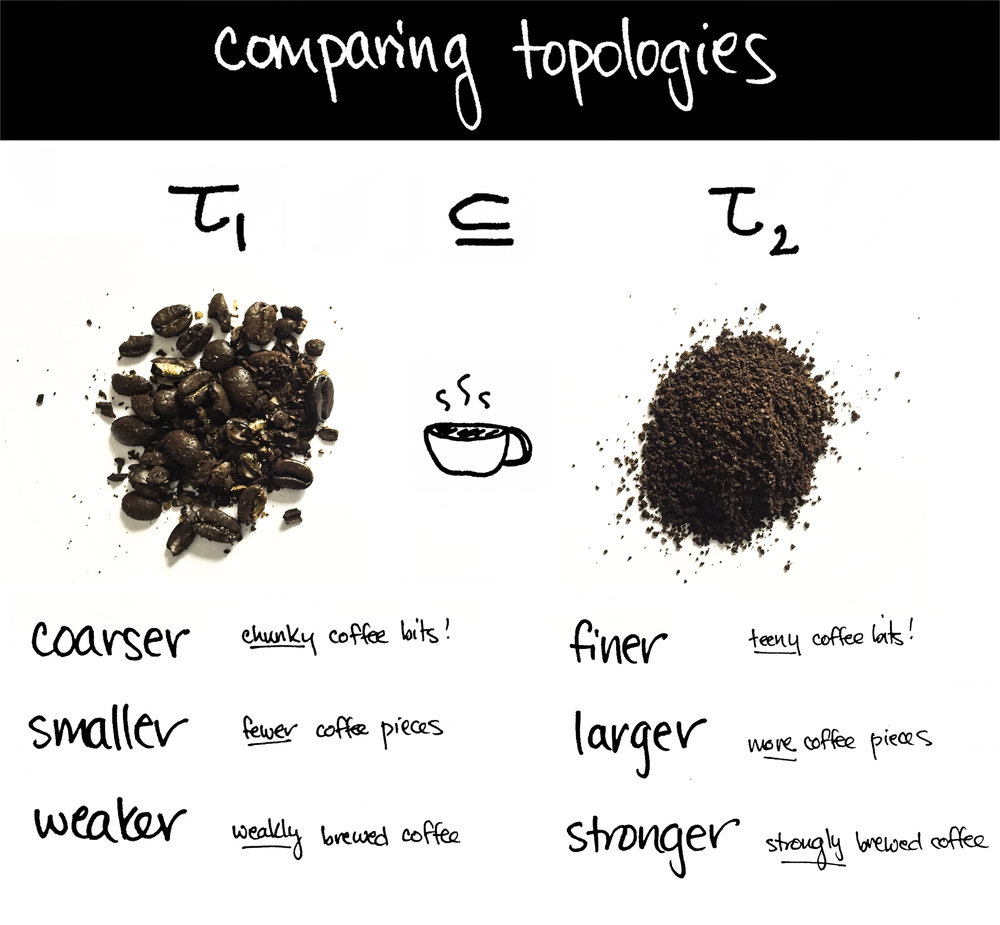
\includegraphics[width=0.65\linewidth]{pics/comparing-topologies-and-coffee.jpg}
    \caption{Comparing topologies and coffee (Credit:
    \href{http://www.math3ma.com/the-back-pocket/2016/8/26/comparing-topologies}{math3ma})}
\end{figure}
For example, assuming we have
\begin{equation}
    f: X\to Y
\end{equation}
where $f$ is any function.

If $X$ has topolgy $\mathcal{T}_X$, we ask then what kind of topolgy on
$Y$ will make $f$ a continuous function. First, all $f^{-1}(V)$, with
$V\in \mathcal{T}_Y$ should be open in $X$. So, the easiest choice is to
make $\mathcal{T}_{Y,\text{min}}=\{\varnothing,Y\}$, this is the
smallest topolgy.  Also, any set $V\in Y$ such that $f^{-1}(V)\notin
\mathcal{T}_X$ should not be in $\mathcal{T}_Y$. Then the largest
topolgy is $\mathcal{T}_{Y,\text{max}}=\{ V\subset Y| f^{-1}(V)\in
\mathcal{T}_X\}$.

If $Y$ has topolgy $\mathcal{T}_Y$, we also ask what kind of topolgy
on $X$ will make $f$ a continuous function. First, all $V\in
\mathcal{T}_Y$, their preimage $f^{-1}(V)$ must be in $\mathcal{T}_X$.
So the smallest topolgy is
$\mathcal{T}_{X,\text{min}}=\{f^{-1}(V)|V\in\mathcal{T}_Y\}$. Than
what about the largest topolgy? We consider, what kind of sets cannot
be inside $\mathcal{T}_X$. First, can $(f^{-1}(V))^c=f^{-1}(V^c)$ be
in $\mathcal{T}_X$? Yes. Since unless the space is connected, there
can be sets being both open and closed (other than $X$ and
$\varnothing$). Any other restrictions? No that I can think of. So,
the largest topolgy $\mathcal{T}_{X,\text{max}}=2^X$, the set of all
subsets of $X$. (The notation \nomen{$2^X$} is taken from the page 4
of book \cite{Singer.Thorpe}.

A summary:
\begin{table}[H]
    \centering
    \caption{Largest and Smallest Topolgies}
    \begin{tabular}{c l l}
        $X\overset{f}{\to}Y$ & Smallest  &Largest \\
        \hline
        Given $\mathcal{T}_X$ & $\mathcal{T}_{Y,\text{min}}=\{\varnothing,Y\}$        & $\mathcal{T}_{Y,\text{max}}=\{ V\subset Y| f^{-1}(V)\in \mathcal{T}_X\}$\\
        Given $\mathcal{T}_Y$ & $\mathcal{T}_{X,\text{min}}=\{f^{-1}(V)|V\in\mathcal{T}_Y\}$ & $\mathcal{T}_{X,\text{max}}=2^X$ \\
        No constraint & $\{\varnothing,X\}$ & $2^X$ \\
        \hline
    \end{tabular}
\end{table}
\paragraph{Facts about subspace/induced topolgy}
Let $Y$ be a subspace of a topological space $X$ wit induced topolgy.
\begin{fact}
    A set $H\subseteq Y$ is open in $Y$ if and only if $H=F\cap Y$
    for some open set $F$ in $X$.
\end{fact}
\begin{fact}
    A set $H\subseteq Y$ is closed in $Y$ if and only if $H=F\cap Y$
    for some closed set $F$ in $X$.
\end{fact}
\begin{fact}
    A set $H$ is open/closed in $X$ $\Rightarrow$ $H$ is open/closed
    in $Y$. But the converse may not be true. The converse statement
    depends on whether $Y$ is open or closed in $X$.
\end{fact}
\section{Collection of Theorems in Chapter 4}
\label{sec:Collection-of-Theorems-in-Chapter-4}
\begin{defi}[Identification Topology]
\nomenclature{Identification Topology}{\nomrefpage.}
Let $X$ be a topological space and let $\mathscr{P}$ be a family of
disjoint nonempty subsets of $X$ such that $\cup \mathscr{P}=X$. Such
a family is usually called a partition of $X$. Let $Y$ be a new space
whose points are the members of $\mathscr{P}$. Let $\pi:X\to Y$ sends
each point of $X$ to the subset of $\mathscr{P}$. Define a topolgy
$\mathcal{T}_Y$ on $Y$ to be the largest topolgy such that the $\pi$
is continuous. This $\mathcal{T}_Y$ is called the idetification topolgy.
And $Y$ is called the \nomen{identification space}.
\end{defi}
\begin{center} \begin{tikzcd}[]
    X\ar[r]\ar[rd] & Y\ar[d,equal] \\
    & \mathscr{P}
\end{tikzcd} \end{center}
\begin{thm}
    Let $Y$ be an idetification space defined as above and let $Z$ be
    an arbitrary topological space. A function $f:Y\to Z$ is
    continuous if and ony if the composition $f\circ \pi:X\to Z$ is
    continuous.
\end{thm}
\begin{center} \begin{tikzcd}[]
    X\ar[r,"\pi"]\ar[rd]\ar[rr,"f\circ\pi",bend left=30] & Y\ar[d,equal]\ar[r,"f"] & Z \\
    & \mathscr{P}
\end{tikzcd} \end{center}
\begin{defi}[Identification Map]
\nomenclature{Identification Map}{\nomrefpage.}
    Let $f:X\to Y$ be an onto continuous map and suppose that the topolgy on $Y$
    is the largest for which $f$ is continuous. Then we call $f$ an
    identification map.
\end{defi}
The naming "identification map" is because:
\begin{thm}
    Any function $f:X\to Y$ gives rise to a partition of $X$ whose
    members are the subsets $\{f^{-1}(y)\}$, where $y\in Y$. Let $Y_*$
    denote the identification space associated with this partition,
    and $\pi:X\to Y_*$ the usual continuous map. 
    $$ \begin{tikzcd}[]
        X\ar[r,"f"]\ar[d,"\pi"] & Y \\
        \{f^{-1}(y)\} \ar[r,equal] & Y_*
    \end{tikzcd} $$
    If $f$ is an identification map, then:
    \begin{enumerate}
        \item the spaces $Y$ and $Y_*$ are homeomorphic;
        \item a function $g:Y\to Z$ is continuous if and only if the
            composition $g\circ f:X\to Z$ is continuous.
    \end{enumerate}
    $$ \begin{tikzcd}[]
        X\ar[r,"f"]\ar[d,"\pi"]\ar[rr,"g\circ f",bend left] 
            & Y\ar[d,equal,"~"]\ar[r,"g"] & Z \\
        \{f^{-1}(y)\} \ar[r,equal] & Y_*
    \end{tikzcd} $$
\end{thm}
\begin{thm}
    Let $f:X\to Y$ be an onto continuous map. If $f$ maps open sets of
    $X$ to open sets of $Y$, or closed sets to closed sets, then $f$
    is an identification map, i.e. $\mathcal{T}_y$ is the largest
    topolgy such that $f$ is continuous.
\end{thm}
\begin{coro}
    \label{coro:idmap-coro}
    Let $f:X\to Y$ be an onto continuous map. If $X$ is compact and
    $Y$ is Hausdorff, then $f$ is an identification map.
\end{coro}

\begin{defi}[Torus]
\nomenclature{Torus}{\nomrefpage.}
Torus is the uTorusquare $[0,1]\times[0,1]$, with 1. opposite edge
identified, 2. four edge points identified.
\end{defi}
\begin{remark}
    The identification map and corollary \ref{coro:idmap-coro} can be
    used to show that torus is homeomorphic to two copies of
    circles:$S^1\times S^1$. This is mentioned in page 68 of
    \cite{book}.
\end{remark}
\begin{defi}[Cone $CX$]
\nomenclature{Cone $CX$}{\nomrefpage.}
    The cone of any space $CX$ is formed from $X\times I$, where $I$ is
    the unit interval $[0,1]$, with certain identification. The
    identification shrinks all points in one surface into one point.
    This is discussed in page 68 of \cite{book}.
\end{defi}
\begin{figure}[H]
    \centering
    \includegraphics[width=0.5\linewidth]{pics/{Cone-of-a-circle}.pdf}
    \caption{Cone of a Circle (Wikipedia)}
\end{figure}
\begin{remark}
    There is another definition of cone $CX$ when $X$ in imbeded into
    $\mathbb{E}^n$, may be found on page 68 of \cite{book}. Cone
    constructed in this way is called a geometric cone. It is made up
    of all straight line segments that join $v=(0,0,\cdots,1)\in
    \mathbb{E}^{n+1}$ to some point of $X$.
\end{remark}
\begin{lemma}
    The geometric cone on $X$ is homeomorphic to $CX$.
\end{lemma}
\begin{defi}[Quotient Space]
\nomenclature{Quotient Space}{\nomrefpage.}
    Let $X$ be a topological space, $A$ be its subspace. Then $X/A$
    menas the $X$ with subspace $A$ identified to a point.
    \begin{enumerate}
        \item the set $A$.
        \item the individual points of $X\setminus A$.
    \end{enumerate}
\end{defi}
\begin{remark}
    In this notation, $CX$ becomes $(X\times I)/(X\times\{1\})$.
\end{remark}
\begin{fact}
    \begin{equation}
        B^n/S^{n-1} \cong S^n
    \end{equation}
    where $\cong$ menas homeomorphic. This is proved on page 69.
    Intuitively, this is like wrap a lower dimension ball surround the
    higher dimension ball.
\end{fact}

\begin{defi}[$f\cup g$]
\nomenclature{$f\cup g$}{\nomrefpage.}
    Let $X,Y$ $f\cup g$ subsets of a topological space and give each of
    $X,Y$, and$X\cup Y$ the induced topolgy. If $f:X\to Z$ and
    $g:Y\to Z$ are functions which agree on the intersection of $X$
    and $Y$, we can define
    \begin{align}
        f\cup g &: X\cup Y \to Z  \\
        (f\cup g)(x) &= f(x),\, x\in X \nonumber \\
        (f\cup g)(x) &= g(x),\, x\in Y \nonumber
    \end{align}
    We say that $f\cup g$ are formed by 'glueing together' the
    functions $f$ and $g$.
\end{defi}
\begin{lemma}[Glueing lemma (closed)]
    If $X$ and $Y$ are closed in $X\cup Y$, and if both $f$ and $g$
    are continuous, then $f\cup g$ are continuous.
\end{lemma}
Similarly, 
\begin{lemma}[Glueing lemma (open)]
    If $X$ and $Y$ are open in $X\cup Y$, and if both $f$ and $g$
    are continuous, then $f\cup g$ are continuous.
\end{lemma}

These two lemmas are seen as a special case of the following theorem,
explained in page 70.

Define \nomen{$X+Y$} to be the disjoint union of spaces $X,Y$. Define
$j:X+Y \to X\cup Y$ which restrict to either $X$ or $Y$ is just the
inclusion in $X\cup Y$.
\begin{thm}
    If $j$ is an identification map, and if both $f:X\to Z$ and
    $g:X\to Z$ are continuous, then $f\cup g:X\cup Y\to Z$ is
    continuous.
\end{thm}
$$ \begin{tikzcd}[]
    X+Y \ar[r,"j"] & X\cup Y\ar[r,"f\cup g"] & Z \\
    X\ar[rru,"f"] & Y\ar[ru,"g",bend right]
\end{tikzcd}$$

This can be generalized as follows. Let $X_\alpha,\alpha\in A$ be a
family of subsets of a topological space and give each $X_\alpha$ and
the union $\cup X_\alpha$, the induced topolgy. Let $Z$ be a space and
suppose we are given maps $f_\alpha:X_\alpha\to Z$, one for each
$\alpha$ in $A$, such that if $\alpha,\beta\in A$,
$$ 
\eval{f_\alpha}_{X_\alpha\cap X_\beta} = \eval{f_\beta}_{X_\alpha\cap X_\beta}
$$
Define function $F:\cup X_\alpha\to Z$ by glueing together $f_\alpha$.
Let $\oplus X_\alpha$ be the disjoint unin of spaces $X_\alpha$. Let
$j:\oplus X_\alpha \to \cup X_\alpha$ be similarly defined.
\begin{thm}
    If $j$ is an identification map, and if each $f_\alpha$
    is continuous, then $F$ is continuous.
\end{thm}
\textbf{Note}: When $j$ is the identification map, then $\cup
X_\alpha$ has the identification topolgy instead of the subspace
topology. The two will be quite different, as discussed on page 70 to
71 of \cite{book}.

\begin{defi}[Projective space $P^n$]
\nomenclature{Projective space}{\nomrefpage.}
    A discussion of real $P^n$ may be found on page 71.
\end{defi}

\paragraph{\nomen{Attaching maps} and $X\cup_f Y$} Let:
\begin{equation}
    Y \supseteq A \overset{f}{\to} X
\end{equation}
where $X,Y$ are topological spaces, $f$ is continuous. We identify the
disjoint union $X+Y$ using $f$, partitioning them into:
\begin{enumerate}
    \item pairs of points $\{a,f(a)\}$ where $a\in A$;
    \item individual points of $Y\setminus A$;
    \item individual points of $X\setminus \Im(f)$.
\end{enumerate}
The result identification space is denoted $X\cup_f Y$, and $f$ is
called the attaching map. This process can also be viewed as:
\begin{equation}
    X\cup_f Y = (X\amalg Y)/\{f(A)~A\}
\end{equation}
\begin{figure}[H]
    \centering
    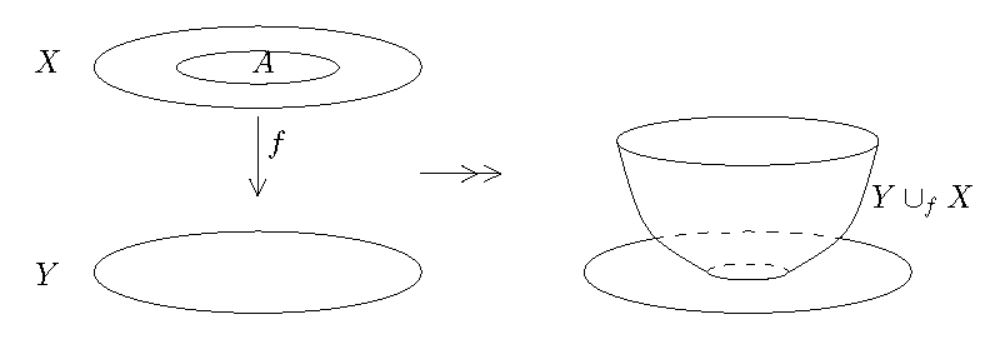
\includegraphics[width=0.6\linewidth]{pics/Attaching-Space.jpg}
    \caption{Attaching Space (credit:
        \href{https://ncatlab.org/nlab/show/Top}{nLab}}
\end{figure}
\begin{ex}
    $P^2$ can be seen as attaching a closed disc $D$ to the boundary
    of $M$, a Mobius strip, as discussed in page 72 of \cite{book}.
    Geometrically, this simply shrinks the boundary of $M$ into a
    point. And an ant travelling around this point can point out the
    direction just as in $P^2$.
\end{ex}
\begin{remark}
    It is remarked that properties such as compactness, connectedness,
    and path-connectedness is inherited in identification. However,
    Hausdorff-ness is not. An counter example can be found in page 72 of
    \cite{book}.
\end{remark}
\section{Anchor}
\label{sec:Anchor}

\begin{thebibliography}{1}
    \bibitem{book} M.A. Armstrong. Basic Topology. 2ed.
    \bibitem{Singer.Thorpe} I.M. Singer, J.A. Thorpe. Lecture Notes on
    Elementary Topology and Geometry. UTM.
\end{thebibliography}
\printnomenclature
\section{License}
The entire content of this work (including the source code
for TeX files and the generated PDF documents) by 
Hongxiang Chen (nicknamed we.taper, or just Taper) is
licensed under a 
\href{http://creativecommons.org/licenses/by-nc-sa/4.0/}{Creative 
Commons Attribution-NonCommercial-ShareAlike 4.0 International 
License}. Permissions beyond the scope of this 
license may be available at \url{mailto:we.taper[at]gmail[dot]com}.
\end{document}
